
\chapter{Architettura}


% Un algoritmo si dice \emph{online} se processa il suo input pezzo dopo pezzo in modo sequenziale, cio\`e nell'ordine nel quale l'input viene dato all'algoritmo. L'algoritmo deve produrre risultati a priori cio\`e anche senza avere a disposizione l'intero input fin dall'inizio. D'altro canto un algoritmo si dice \emph{offline} se pu\`o produrre una risposta anche dopo aver analizzato tutto il suo input. Per sua natura un algoritmo online deve fare delle scelte parziali. 

\section{Componenti}

\begin{figure}
  \centering
  %  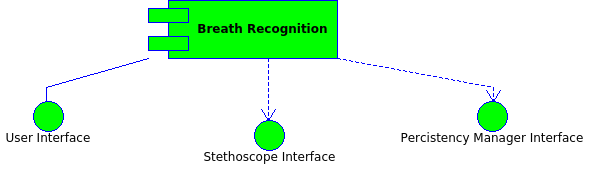
\includegraphics[width=\textwidth,height=0.4\textheight]{./componentdiagram.png}
  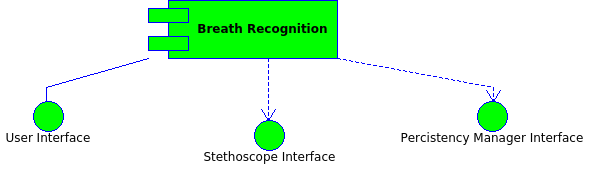
\includegraphics[width=0.8\textwidth]{./componentdiagram.png}
  % componentdiagram.png: 963x508 pixel, 96dpi, 25.48x13.44 cm, bb=0 0 722 381
  \caption{Diagramma delle componenti del sistema}
  \label{componentiSistemaArchitettura}
\end{figure}

Il sistema di monitoraggio ha le componenti illustrate nella figura \ref{componentiSistemaArchitettura}. Discutiamo di ognuna di esse pi\`u in dettaglio nel seguito del capitolo

\subsection{Meccanismi di persistenza}

Il sistema implementa dei meccanismi di persistenza. Un interfaccia minimale di una componente che implementa un meccanismo di persistenza deve offrire le operazioni seguenti:
\begin{itemize}
  \item 
    Aggiungere i dati di nuovo soggetto.
  \item
    Aggiungere una entry di dati di un monitoraggio relativa ad un certo soggetto.
  \item
    Cercare una entry di dati di un monitoraggio a partire dai dati del soggetto e/o dalla data del monitoraggio.
  \item
    Reperire una entry di dati di un monitoraggio a partide da una chiave cercata in precedenza.
\end{itemize}

% Siamo di fronte ad un classico caso di tipo di dato astratto memoria associativa. 
La figura \ref{pppppp} elenca alcuni possibli modi di implementare questo meccanismo di persistenza.


\begin{figure}
  \centering
  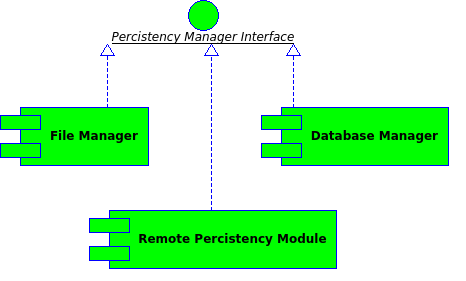
\includegraphics{./persistencyManagerInterface.png}
  % persistencyManagerInterface.png: 466x281 pixel, 96dpi, 12.33x7.43 cm, bb=0 0 349 211
  \caption{Possibili componenti che implementano l'interfaccia con un meccanismo di persistenza}
  \label{pppppp}
\end{figure}

% \begin{figure}
%  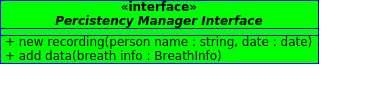
\includegraphics{./persistencyManagerInterfaceOperations.png}
%  % persistencyManagerInterfaceOperations.png: 382x92 pixel, 96dpi, 10.11x2.43 cm, bb=0 0 286 69
%   \label{persistencyManagerInterfaceOperations}
%   \caption{Interfaccia del meccanismo di persistenza}
% \end{figure}

I dati persistenti sono: il nome del sogetto, la data, l'indice di apnea-ipopnea e una sequenza di etichette nell'insieme: respiro o pausa respiratoria. Ogni etichetta corrisponde a $4s$ di segnale. 
% \paragraph{$File\; nella\; memoria\; di\; massa$}
  Il sistema permette di salvare i dati di un monitoraggio sulla memoria di massa del computer sotto forma di file. Vengono usati i meccanismi di serializzazione offerti da Java. La serializzazione di Java permette di memorizzare e leggere uno stream di oggetti Java\cite{javaSerializable}. 
  Per ottimizzare questa operazione, i dati vengono memorizzati prima in un buffer, quando il buffer si riempe vengono scritti sulla memoria di massa. 
  Anche se questa ottimizzazione pu\`o sembrare inutile in quanto tutti i file system moderni sfruttano un meccanismo implicito di buffering, la dimensione di quest'ultimo potrebbe avere un valore predefinito troppo piccolo.


% \paragraph{$Database$}
% Decidere e descrivere cosa come e dove viene memorizzato(tabelle e campi)


% sogetto(
%   nome completo VARCHAR(50),
%   data di nascita DATE,
%   registrazioni: nome di una tabella che contiene tutti i riferimenti alle registrazioni relative a questo soggetto
% )
% 
% persone(
%     id ID,
%     nome completo VARCHAR(50),
%     data di nascita DATE,
%     luogo di nascita VARCHAR(50),
%     luogo di residenza VARCHAR(50),
%     PRIMARY KEY (nome completo, data di nascita, luogo di nascita, id unico)
% )
% 
% registrazioni(
%   soggetto riferimeto a persone
%   
% )






\subsection{Interfaccia con lo stetoscopio}



In generale i sistemi di monitoraggio continuo di parametri fisiologici hanno bisogno di interfacciarsi con i sensori di interesse. 
Questo sistema non \`e una eccezione. 
Riteniamo che una interfaccia minima con lo stetoscopio elettronico sia quella illustrata nella figura \ref{interfacciastetoscopiominima}. Le operazioni illustrate sono:
\begin{description}
  \item[$connect$]
    Inizializza la connessione con il sensore ed allocare eventuali risorse necessarie.
  \item[$disconnect$]
    Terminare la connessione con il sensore e deallocare eventuali risorse.
  \item[$read$]
    Legge $length$ campioni di input e li memorizza nel buffer a partire dall'offset specificato.
  \item[$skip$]
    Tralascia un certo numero di campioni. Puo' essere utile per recuperare in parte un eventuale ritardo globale.
\end{description}



\begin{figure}
\centering
  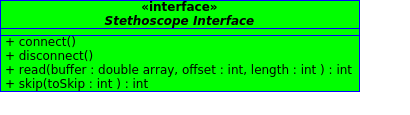
\includegraphics{./stethoscopeInterfaceOperations.png}
% stethoscopeInterfaceOperations.png: 410x115 pixel, 96dpi, 10.85x3.04 cm, bb=0 0 307 86
\caption{Operazioni dell'interfaccia con lo stetoscopio}
\label{interfacciastetoscopiominima}
\end{figure}



Il sistema deve includere almeno una componente che implementa l'interfaccia tra il dispositivo di monitoraggio e il sensore.
Alcune opzioni sono illustrate in figura \ref{componentiinterfacciastetoscopiominima}.

  \begin{figure}
  \centering
 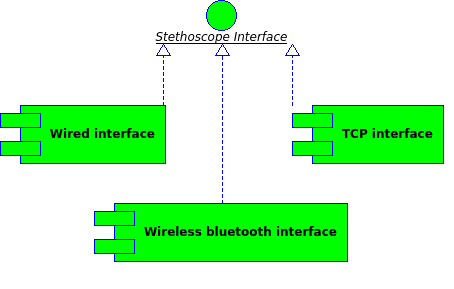
\includegraphics{./stethoscopeInterfaceComponent.png}
 % stethoscopeInterfaceComponent.png: 454x289 pixel, 96dpi, 12.01x7.65 cm, bb=0 0 340 217
  \caption{Possibili componenti che implementano l'interfaccia con lo stetoscopio}
  \label{componentiinterfacciastetoscopiominima}
  \end{figure}

Ci sono appunto vari modi di implementare una connessione tra lo stetoscopio e il dispositivo di monitoraggio. Una scelta che dobbiamo fare riguarda il mezzo di trasmissione del segnale:
\begin{description}
  \item[via cavo]
    In questa modalit\`a spesso \`e necessaria la presenza di personale medico specializzato. Tra gli svantaggi di questa impostazione notiamo: ridotta mobilit\`a del sistema, probabile necessit\`a di alimentazione elettrica dalla rete, rischio di gestione inadeguata di contatti nei cavi.
  \item[senza cavo]
    Una connessione senza fili presenta alcuni vantaggi ad esempio permette al paziente di muoversi pi\`u liberamente e i costi di installazione si possono ridurre.
\end{description}

Riteniamo che per questo sistema sia pi\`u adeguata una connessione senza fili. 

Un'altra scelta riguarda il protocollo di comunicazione, il quale per\`o potrebbe dipendere anche dalla scelta del mezzo di trasmissione.

% Streaming media is multimedia that is constantly received by and presented to an end-user while being delivered by a provider. Its verb form, "to stream", refers to the process of delivering media in this manner; the term refers to the delivery method of the medium rather than the medium itself.
% 
% A client media player can begin playing the data (such as a movie) before the entire file has been transmitted. Distinguishing delivery method from the media distributed applies specifically to telecommunications networks, as most other delivery systems are either inherently streaming (e.g., radio, television) or inherently nonstreaming (e.g., books, video cassettes, audio CDs). 
% For example, in the 1930s, muzak was among the earliest popularly available streaming media; nowadays Internet television is a common form of streamed media. 
% The term "streaming media" can apply to media other than video and audio such as live closed captioning, stock ticker, and real-time text, which are all considered "streaming text". 
% The term "streaming" was first used in the early 1990s as a better description for video on demand on IP networks; at the time such video was usually referred to as "store and forward video",[1] which was misleading nomenclature.
% 
% Live streaming, delivering live over the Internet, involves a camera for the media, an encoder to digitize the content, a media publisher, and a content delivery network to distribute and deliver the content.
% 
% 
% A broadband speed of 2.5 Mbit/s or more is recommended for streaming movies, for example to an Roku, Apple TV, Google TV or a Sony TV Blu-ray Disc Player, 10 Mbit/s for High Definition content.[8]
% 
% 
% 
% Unicast connections require multiple connections from the same streaming server even when it streams the same content
% Streaming media storage size is calculated from the streaming bandwidth and length of the media using the following formula (for a single user and file):
% 
% storage size (in megabytes) = length (in seconds) × bit rate (in bit/s) / (8 × 1024 × 1024)[note 1]
% Real world example:
% 
% One hour of video encoded at 300 kbit/s (this is a typical broadband video as of 2005 and it is usually encoded in a 320 × 240 pixels window size) will be:
% 
% (3,600 s × 300,000 bit/s) / (8×1024×1024) requires around 128 MB of storage.
% If the file is stored on a server for on-demand streaming and this stream is viewed by 1,000 people at the same time using a Unicast protocol, the requirement is:
% 
% 300 kbit/s × 1,000 = 300,000 kbit/s = 300 Mbit/s of bandwidth
% This is equivalent to around 135 GB per hour. Using a multicast protocol the server sends out only a single stream that is common to all users. 
% Therefore such a stream would only use 300 kbit/s of serving bandwidth. See below for more information on these protocols.
% 
% The calculation for live streaming is similar.
% 
% Assumptions: speed at the encoder, is 500 kbit/s.
% 
% If the show lasts for 3 hours with 3,000 viewers, then the calculation is:
% 
% Number of MBs transferred = encoder speed (in bit/s) × number of seconds × number of viewers / (8*1024*1024)
% Number of MBs transferred = 500 x 1024 (bit/s) × 3 × 3,600 ( = 3 hours) × 3,000 (nbr of viewers) / (8*1024*1024) = 1,977,539 MB





Siamo in presenza di un problema la cui modellazione porta naturalmente a pensare ad un pattern architetturale di tipo client server. 
Un server \`e un dispositivo fisico o virtuale che possiede una risorsa da condividere\cite{clientServer}, in questo caso il server \`e lo stetoscopio e la risorsa da condividere \`e il suono che esso registra. Un cliente \`e un dispositivo fisico o virtuale che richiede una certa risorsa ad un server\cite{clientServer}, in questo caso il client \`e il dispositivo di analisi del suono.



\paragraph{bluethoot}
In base alle considerazioni fatte da \cite{BBATMBS}, la teconologia wireless bluethoot si adatta bene al nostro sistema. Il bluethoot permette di stabilire semplici connessioni ad hoc tra dispositivi che hanno a disposizione poca energia elettrica e che sono posti a piccola distanza tra di loro, dove per piccola distanza approssimativamente intendiamo che i dispositivi si trovano nella stessa stanza o anche entro certi limiti in una stessa struttura ospedaliera. I valori precisi di consumi, distanze e velocit\`a di trasmissione variano da dispositivo a dispositivo. Lo stetoscopio elettronico invia continuamente dati al sistema di riconoscimento attraverso il canale bluethoot. I dati inviati dipendono dal particolare stetoscopio ma possiamo aspettarci che questi siano sotto forma di pacchetti di un segnale audio digitale. Suggeriamo quindi di implementare il sistema nel modo illustrato nella figura \ref{blueinterfacciastetoscopiominima}
\begin{figure}
 \centering
 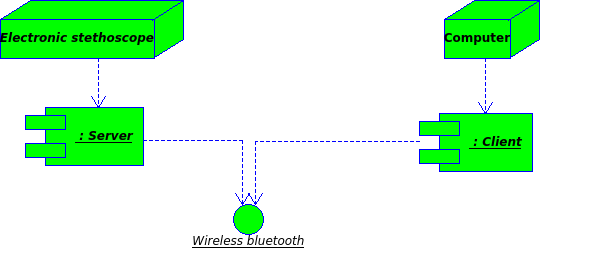
\includegraphics[width=0.9\textwidth]{./deploymentDiagram.png}
 % deploymentDiagram.png: 606x266 pixel, 96dpi, 16.03x7.04 cm, bb=0 0 454 199
  \caption{Architettura del sistema}
  \label{blueinterfacciastetoscopiominima}
\end{figure}


\paragraph{velocit\`a dell'intefaccia}

Supponiamo che il sistema abbia una velocit\`a media di esecuzione di $v_{s}$ campioni di segnale al secondo, e supponiamo che $v$ sia maggiore della frequenza di campionamento e che quindi il sistema riesca ad analizzare un segnale di un secondo in un tempo minore di un secondo. Questa velocit\`a si intende calcolata senza contare il tempo di trasmissione dallo stetoscopio al sistema.

Supponiamo che la velocit\`a di trasmissione dell'interfaccia tra sistema e stetoscopio sia $v_{i}$ bit al secondo e siano $f_{c}$ la frequenza di campionamento del segnale e $size$ la dimensione in bit di un campione di segnale. Allora deve valere
\[
  \displaystyle  \frac{f_{c}}{v_{s}} + \displaystyle \frac{f_{c}}{\left\lfloor\frac{v_{i}}{size}\right\rfloor} \leq 1s
\]
affinch\'e il sistema non accumuli ritardo.













\subsection{Interfaccia utente}



Una interfaccia utente per questo sistema dovrebbe fornire almeno le operazioni elencate nella figura \ref{interfacciautente}.

  \begin{figure}
  \centering
  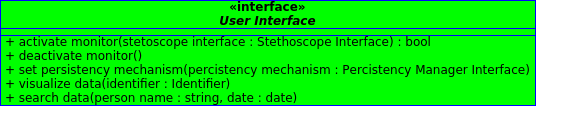
\includegraphics[width=0.8\textwidth]{./userInterfaceOperations.png}
  % userInterfaceOperations.png: 583x138 pixel, 96dpi, 15.42x3.65 cm, bb=0 0 437 103
  \caption{Operazioni dell'interfaccia utente}
  \label{interfacciautente}
  \end{figure}

Sono state implementate due interfacce minimali: 
\begin{description}
  \item[console]
    Un interprete di comandi da console che ha questo aspetto:
    \begin{verbatim}
Breath Monitor Beta version
by Federico Viscomi
type help for a command list

$ help

exit                	exit application             
help                	print this help               
list                	list working directory content
monitor -f filename 	start breath recognition on given file name
stop                	stop current monitoring if any
$ 
    \end{verbatim}

  \item[GUI]
    Una interfaccia grafica basata su Swing \cite{Swing} che offre le stesse funzioni di quella grafica e in pi\`u usa la libreria open source JMathPlot \cite{jmathplot} per disegnare il grafico nel dominio del tempo del segnale. Questo grafico \`e utile solo nella versione iniziale del sistema per motivi di debug. Mentre in una versione successiva del sistema si pu\`o rimpiazzare questo grafico con quello del flusso d'aria. La finestra principale \`e illustrata in figura \ref{finestraprincipale}.
\end{description}

\begin{figure}
 \centering
 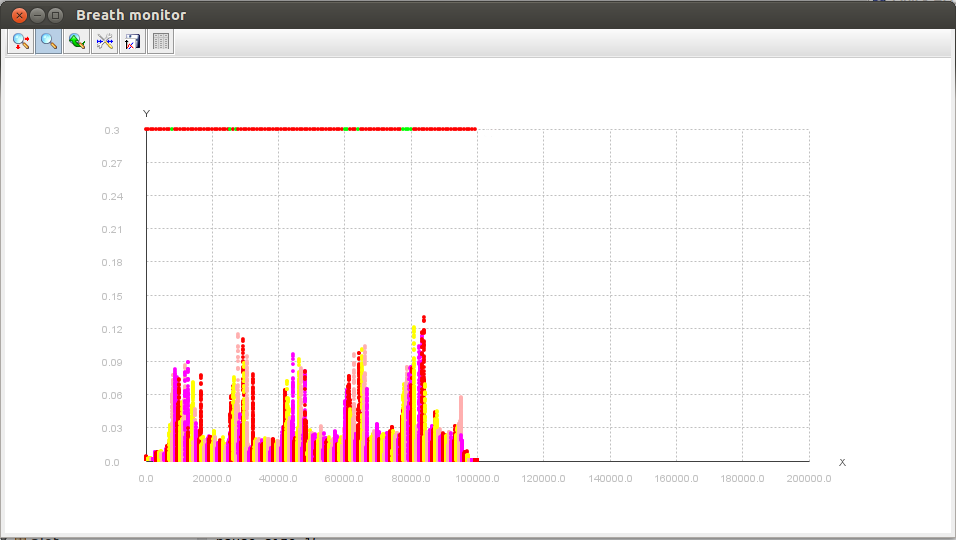
\includegraphics[width=0.8\textwidth]{gui.png}
 % gui.png: 0x0 pixel, 0dpi, 0.00x0.00 cm, bb=
  \label{finestraprincipale}
\end{figure}



